% !TeX root = ./main.tex

Each explanation in the sequence will be non-redundant and hence as small as possible. Yet, in our earlier work we noticed that some explanations were still quite hard to understand, mainly since a clue had to be combined with implicit constraints and a couple of previously derived facts. All these things \textit{together} implied a consequence, and they had to be taken into account at once.
Such steps turned out to be too complicated to be understood easily and thus require being explained in more detail.

An example is depicted at the top in Figure \ref{fig:pasta_diff}.
It uses a disjunctive clue (``The person who ordered Rotini is either the person who paid \$8 more than Damon or the person who paid \$8 less than Damon''), in combination with three previously derived facts to derive that Farfalle does not cost \$8.
This derivation is non-trivial, but can be explained in a step-wise manner using reasoning by contradiction:
\begin{itemize}
    \item If Farfalle did cost \$8, then (since Damon did not eat Farfalle), Damon did not pay \$8;
    \item If Farfalle costs \$8, then it does not cost \$16;
    \item Since Farfalle does not cost \$16 and neither does Capellini or Tagliolini, Rotini must cost \$16;
    \item However, the fact that Rotini costs \$16, while Damon did not pay \$8 is in contradiction with the clue in question;
    \item Hence, Farfalle can not cost \$8.
\end{itemize}
The reasoning step in this Figure~\ref{fig:pasta_diff} is equally straightforward for a computer as the bijectivity reasoning step in Figure~\ref{fig:zebrascreen}. However, understanding the former reasoning step is notably harder for a person.

\begin{figure}[t!]
    \centering
    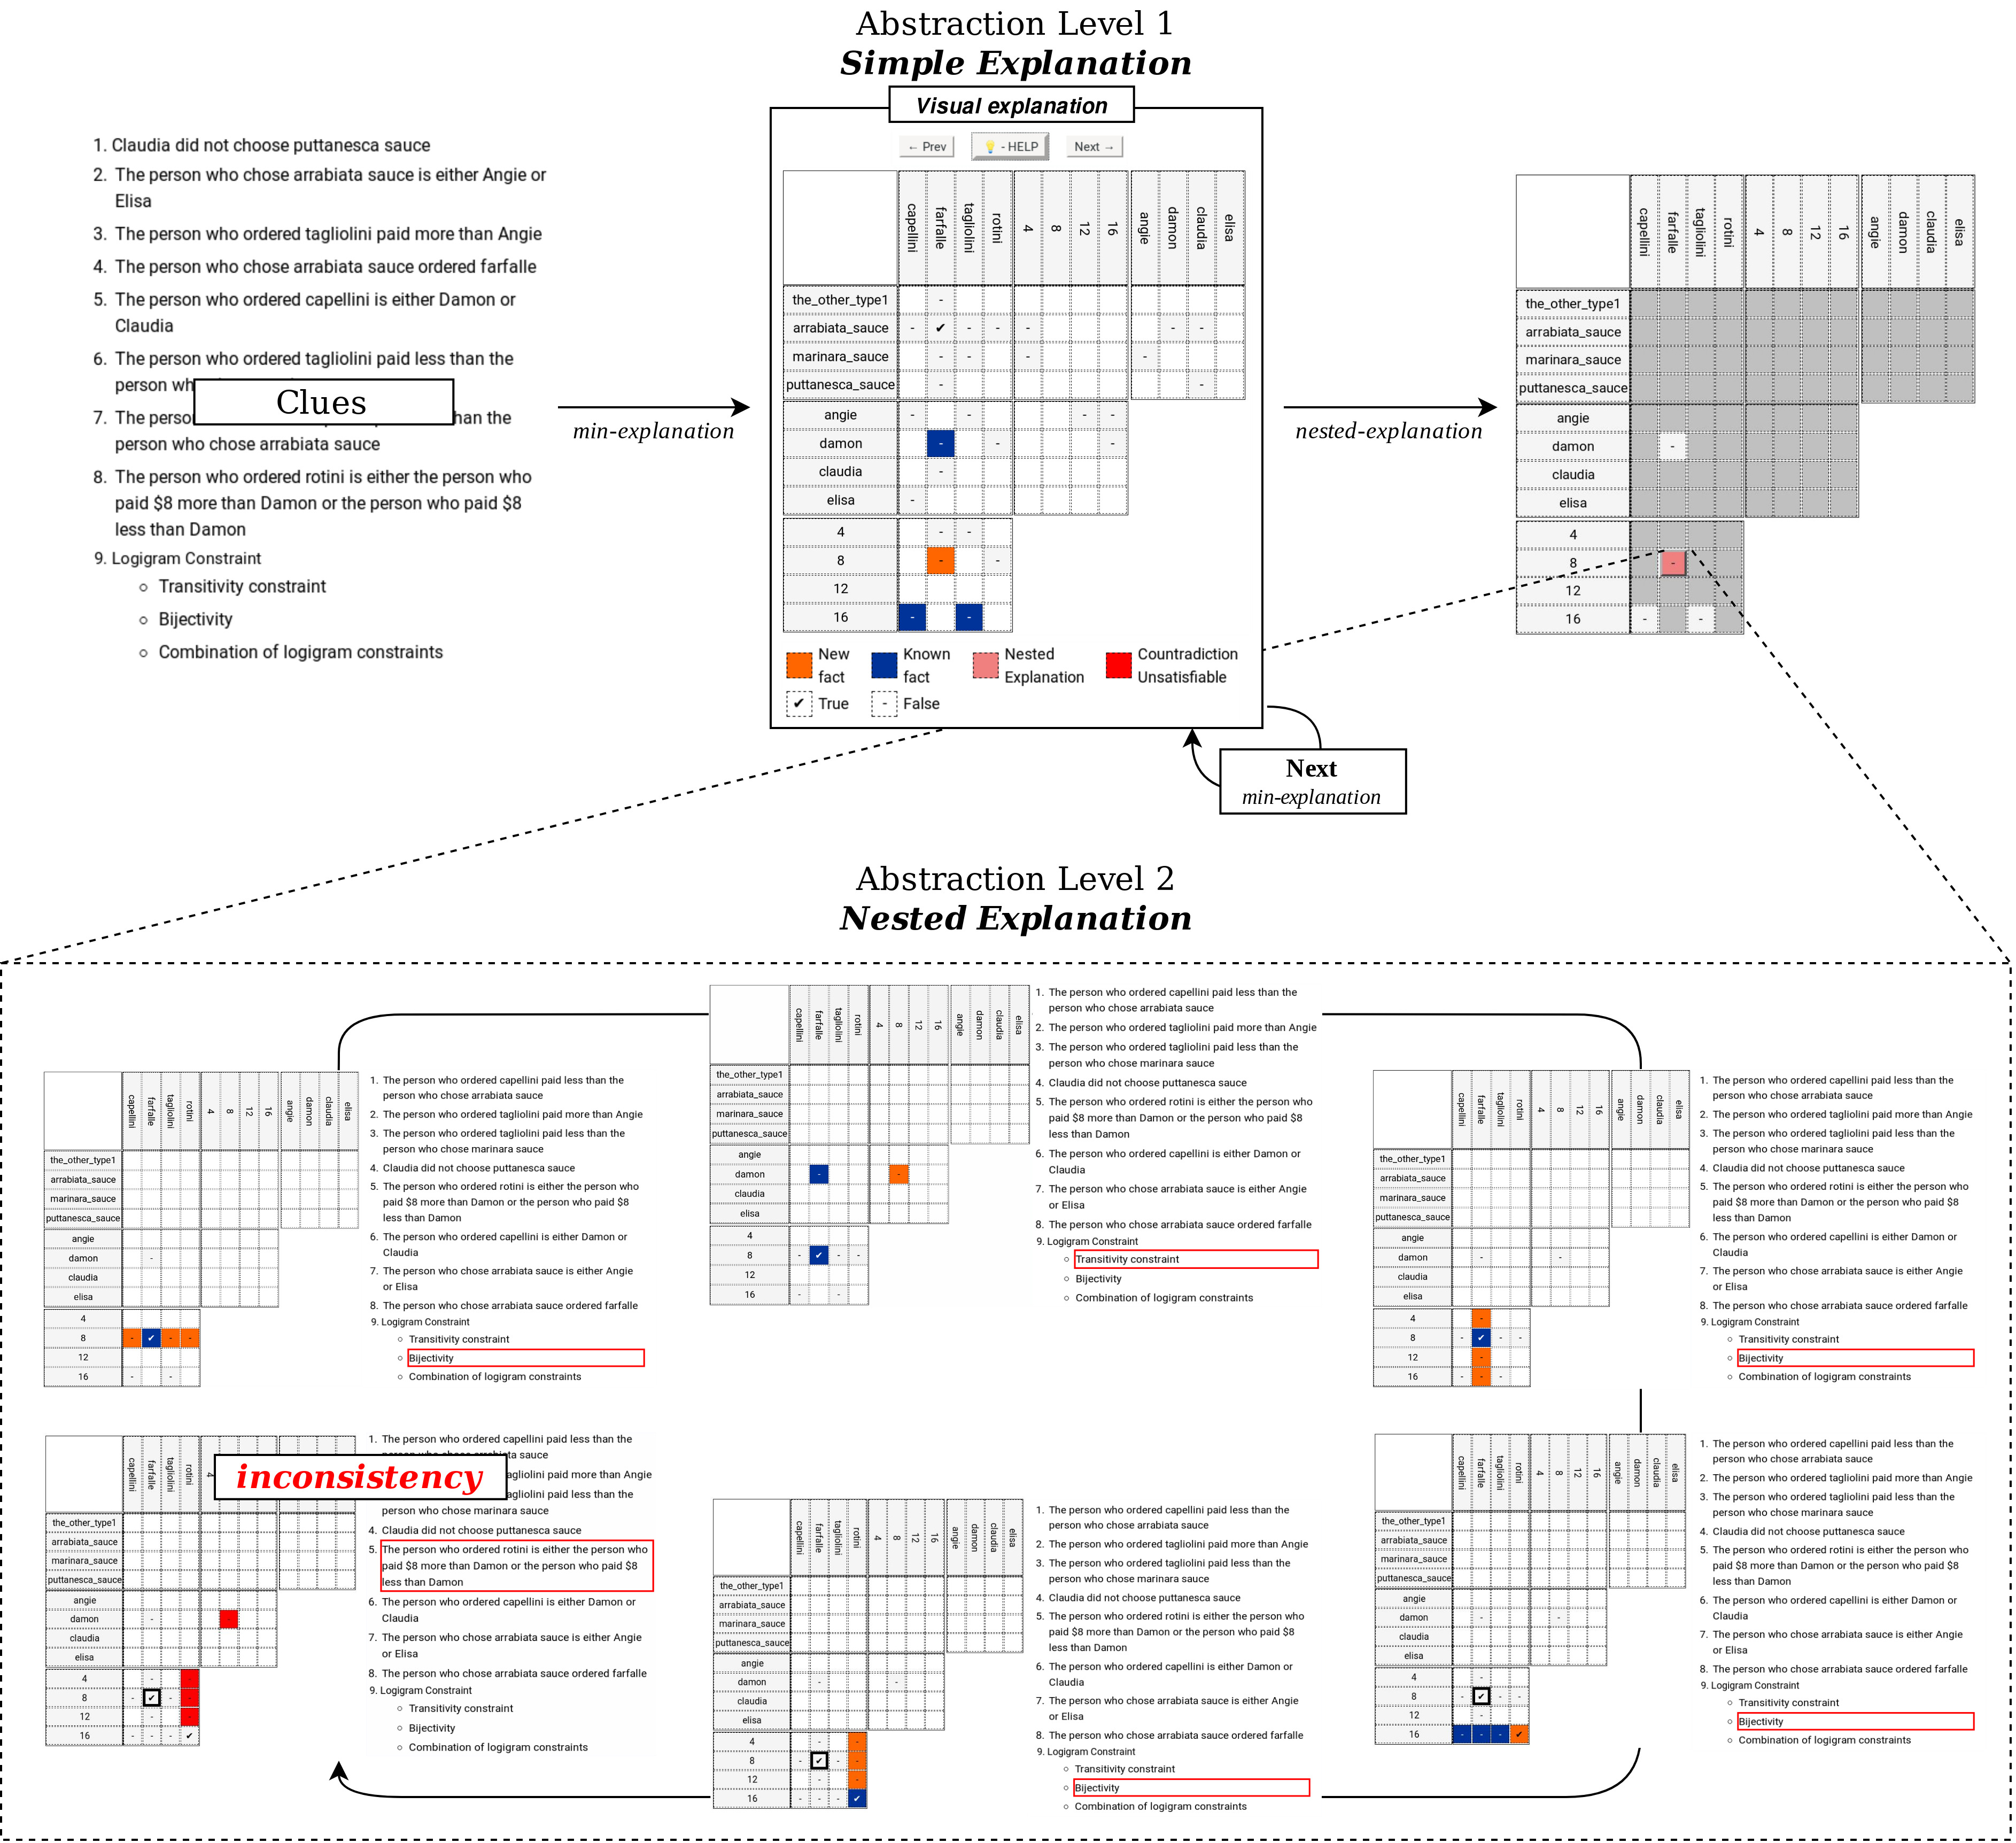
\includegraphics[width=\textwidth]{figures/inconsistency.jpg}
    \caption{A difficult explanation step, including its nested explanation}\label{fig:pasta_diff}
\end{figure}

We hence wish to provide a further, \textit{nested} explanation of such difficult reasoning steps. We believe that an explanation using contradiction is a good tool for this for two reasons: \emph{(i)} it is often used by people when solving puzzles, as well as by mathematicians when proving theorems; and \emph{(ii)} adding the negation of a derived fact such as `Farfalle does not cost \$8', allows us to generate a new sequence of non-redundant explanations up to inconsistency and hence contradiction, hence reusing the techniques from the previous section.
This novel approach allows us to provide a mechanism for \emph{zooming in} into the most difficult explanation step.

\myparagraph{Nested explanation of a reasoning step}

We propose the following principles for what constitutes a meaningful and simple nested explanation, given a non-trivial explanation $(E,S,N)$:
\begin{itemize}
    \item a nested explanation starts from the explaining facts $E$,
          augmented with the counterfactual assumption of a newly derived fact $n \in N$;
    \item at each step, it only uses clues from $S$;
    \item each step is easier to understand (has a strictly lower cost) than the parent explanation with cost $f(E,S,N)$;
    \item from the counterfactual assumption, a contradiction is derived.
\end{itemize}

Note that if an explanation steps derives multiple new facts, e.g. $|N| > 1$, then we can compute a nested explanation for each $n_i \in N$.

More formally, we define the concept of \emph{nested explanation} as follows:

\begin{definition}\label{def:nested-problem}
    The \textbf{nested explanation} problem consists of --- given a non-redundant explanation $(E, S, N)$, and a newly derived fact $n \in N$ --- finding a non-redundant explanation sequence
    \[\langle \ (I_0',(\emptyset,\emptyset,\emptyset)),\ (I_1',(E_1',S_1',N_1')), \dots ,\ (I_n',(E_n',S_n',N_n')) \ \rangle\]
    such that:
    \begin{itemize}
        \item $I_0'$ is the partial interpretation $\{ \neg n_i \wedge E \}$;
        \item $S_i'\subseteq S$ for each $i$;
        \item $f(E_i',S_i',N_i')< f(E, S, N)$ for each $i$;
        \item $I_n'$ is inconsistent; and
        \item a predefined aggregate over the sequence $\left(f(E_i',S_i',N_i')\right)_{i\leq n}$ is minimised.
    \end{itemize}
\end{definition}

We can hence augment each explanation $(E,S,N)$ with a set of nested explanations if they exist. We next discuss algorithms for computing explanations and nested explanations.
